\clearpage\begingroup
\hypertarget{native-283-21}{}
\HistoricalHead{278}{L}{PRAKTISCHE UND SPHÄRISCHE ASTRONOMIE. BRIEFWECHSEL.}
\begin{center}[21.]\quad \textsc{Gauss} an \textsc{Olbers}, 11. November 1835.\end{center}
\begin{center}\small
\rule{.92\textwidth}{.35pt}\\[.2em]
\textsc{Wilhelm Olbers}, Sein Leben und seine Werke, II\textsubscript{2}, Berlin 1909, S. 628.\\[-.2em]
\rule{.92\textwidth}{.35pt}
\end{center}
\noindent\begin{minipage}[t]{.16\textwidth}
\vspace*{7\baselineskip}
\centering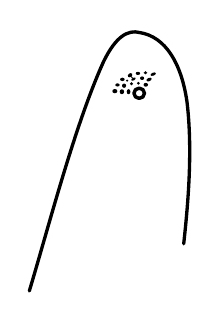
\begin{tikzpicture}[x=.167pt,y=-.167pt,line cap=round,line join=round]
\draw[line width=1.2pt] (0,560)
 .. controls (43,417) and (99,199) .. (161,63)
 .. controls (187,10) and (213,-6) .. (239,1)
 .. controls (295,10) and (329,68) .. (341,150)
 .. controls (353,249) and (345,359) .. (334,458);
\draw[line width=1.25pt] (237.7,132.3) ellipse[x radius=1.9pt,y radius=1.85pt];
\fill (235,89.3) ellipse[x radius=.80pt,y radius=.57pt];
\fill (251.3,88) ellipse[x radius=.66pt,y radius=.58pt];
\fill[rotate around={22:(268,91)}] (268,91) ellipse[x radius=1.03pt,y radius=.53pt];
\fill[rotate around={39:(218,93.3)}] (218,93.3) ellipse[x radius=.89pt,y radius=.66pt];
\fill[rotate around={28:(225.3,101.7)}] (225.3,101.7) ellipse[x radius=.87pt,y radius=.46pt];
\draw[line width=.28pt] (220,96)--(223.7,99.8);
\fill (201.3,102.3) ellipse[x radius=.83pt,y radius=.61pt];
\fill (211.7,105) ellipse[x radius=.43pt,y radius=.42pt];
\fill (244,99.7) ellipse[x radius=.76pt,y radius=.65pt];
\fill[rotate around={24:(259,102.7)}] (259,102.7) ellipse[x radius=1.00pt,y radius=.60pt];
\fill (221,111.7) ellipse[x radius=.59pt,y radius=.58pt];
\fill (236,110.7) ellipse[x radius=.55pt,y radius=.54pt];
\fill (252,114) ellipse[x radius=.82pt,y radius=.70pt];
\fill (190.7,114.3) ellipse[x radius=.80pt,y radius=.57pt];
\fill (205,116) ellipse[x radius=.75pt,y radius=.78pt];
\fill (185,127.7) ellipse[x radius=.91pt,y radius=.77pt];
\fill (200.3,129) ellipse[x radius=.81pt,y radius=.90pt];
\fill (214.7,129) ellipse[x radius=.67pt,y radius=.91pt];
\end{tikzpicture}

\end{minipage}\hfill
\begin{minipage}[t]{.80\textwidth}
\setlength{\parindent}{1.2em}
\noindent\hspace*{\parindent}\mbox{. . . . . .} Den Cometen [1835 III Halley] habe ich nur wenige Male beobachten können; in der günstigen Zeit habe ich ihn auch nur einmal gesehen, wo sein Anblick etwas sehr Auffallendes darbot. Es war (ich glaube am 12. Oct., doch schreibe ich in diesem Augenblick nur aus dem Gedächtniss) ein sehr heller und \textls[120]{sehr} kleiner Kern da, der aber nach dem Scheitelpunkt des parabolischen Schweifs zu, obwohl nicht genau, sondern etwas seitwärts, einen fächerartigen Auswuchs hatte, etwa wie ein Kreissektor von $120^0$, viel heller als der Schweifstoff, aber viel schwächer als der Kern, und eher \textls[120]{rothgelb}, während der Kern weissgelb war. Leider habe ich dies nur einige Minuten beobachtet, da mein Vorsatz, an spätern Abenden eine ganz besondere Aufmerksamkeit darauf zu richten, durch das stets ungünstige Wetter vereitelt wurde. Ich weiss also garnicht, was ich daraus machen soll. Dr. \textsc{Goldschmidt} und meine Tochter sahen es ganz ebenso wie ich. Die grosse Helligkeit des Kerns machte mir Hoffnung, den Cometen bei \textls[120]{Tage} sehen zu können; ich habe ihm mehrere Male im Meridian aufgepasst, aber immer vergeblich, wiewohl auch jedesmal die Luft etwas dunstig war.
\end{minipage}
\clearpage\endgroup
